%% ============================================================
%%  Beamer slides — Extension v5 (CSP styled)
%%  Supervisor discussion deck, v1..v5 tracking
%%  Compile: pdflatex extension_v5_slides_csp.tex (twice)
%% ============================================================
\documentclass[10pt,aspectratio=169]{beamer}

% ---- CSP style ---------------------------------------------------------
\usepackage{CSPstyles}

% ---- theme: minimal default + CSP palette ------------------------------
\usetheme{default}
\useinnertheme{rectangles}
\setbeamertemplate{navigation symbols}{}
\setbeamertemplate{footline}[frame number]
\setbeamercolor{structure}{fg=CSP-main-dark}
\setbeamercolor{frametitle}{fg=CSP-main-dark}
\setbeamercolor{title}{fg=CSP-main-dark}
\setbeamercolor{subtitle}{fg=CSP-text}
\setbeamercolor{author}{fg=CSP-text}
\setbeamercolor{date}{fg=CSP-text-light}
\setbeamercolor{itemize item}{fg=CSP-main}
\setbeamercolor{itemize subitem}{fg=CSP-main-light}
\setbeamercolor{alerted text}{fg=CSP-emphasis}
\setbeamercolor{normal text}{fg=CSP-text}
\setbeamercolor{block title}{bg=CSP-main-light, fg=CSP-text-dark}
\setbeamercolor{block body}{bg=independence-light-5, fg=CSP-text}
\setbeamerfont{frametitle}{series=\bfseries}
\setbeamerfont{title}{series=\bfseries,size=\LARGE}

% ---- packages ----------------------------------------------------------
\usepackage{booktabs}
\usepackage{array}
\usepackage{graphicx}
\graphicspath{{../05-modelling-production-data/figures/v5/}{../05-modelling-production-data/figures/}{figures/}}
\usepackage{amsmath, amssymb, bm}
\usepackage{colortbl}

% convenience macros (on top of CSPstyles' \emphasis, \accentone, ...)
\newcommand{\main}[1]{\textcolor{CSP-main-dark}{\textbf{#1}}}
\newcommand{\emp}[1]{\textcolor{CSP-emphasis}{\textbf{#1}}}
\newcommand{\acct}[1]{\textcolor{CSP-accent-1-dark}{#1}}      % teal accent
\newcommand{\accy}[1]{\textcolor{CSP-accent-2-dark}{#1}}      % orange/gold
\newcommand{\accg}[1]{\textcolor{CSP-accent-3-dark}{#1}}      % green
\newcommand{\muted}[1]{\textcolor{CSP-text-light}{#1}}

\title{Extension of the RSA Production Model\\
\large Mechanism-level exploration and the $2\!\times\!2$ tradeoff}
\author{Hening Wang}
\date{2026-04-15}

\begin{document}

% ====================================================================
\begin{frame}
\titlepage
\begin{center}
\muted{Branch \texttt{feat/extension-v5} \ \textbullet\  dc subset ($N = 3196$) \ \textbullet\  16 commits}
\end{center}
\end{frame}

% ====================================================================
\begin{frame}{Where we start: the paper-reported model}
\small
Incremental recursive speaker, hierarchical per-participant $\alpha$ offsets. \main{Theory-driven}: minimal parameters with clear motivation.

\vspace{0.4em}
\emp{The $2\!\times\!2$ story (memo \S1)}
\begin{center}
\begin{tabular}{lrrrrr}
\toprule
Model & ELPD LOO & $\Delta$ ELPD & dSE & $\Delta$/dSE & $p$\\
\midrule
\main{Inc.\ recursive} & \main{$-7180$} & $0$ & --- & --- & ---\\
Inc.\ static           & $-7199$ & $-19$  & 1.84  & $-10.28$ & $<.001$\\
Global static          & $-7626$ & $-446$ & 40.27 & $-11.08$ & $<.001$\\
Global recursive       & $-7628$ & $-448$ & 40.69 & $-11.02$ & $<.001$\\
\bottomrule
\end{tabular}
\end{center}

\vspace{0.4em}
\begin{itemize}\itemsep0.25em
  \item \main{Speaker architecture dominates}: inc $\gg$ glb ($\Delta/$dSE $\approx 11$).
  \item \main{Semantic regime within incremental}: recursive $>$ static ($\Delta/$dSE $= 10.28$).
  \item \main{Semantic regime within global}: null.
\end{itemize}
\end{frame}

% ====================================================================
\begin{frame}{But: the fit is poor}
\small
\begin{itemize}\itemsep0.3em
  \item \emp{$R^2 = 0.346$} across the 90 (condition $\times$ utterance) cells.
  \item \emp{L1 aggregate residual $= 3.17$} (cells with emp $\geq 2\%$).
  \item No lapse and no length bias in the reported model --- $\gamma$ and $\varepsilon$ \emph{hardcoded to $0$}. All mass must come from the RSA softmax alone.
\end{itemize}

\vspace{0.5em}
\main{Seven systematic misfits (memo \S5.3)}
\begin{center}\footnotesize
\begin{tabular}{lll rrr}
\toprule
Condition & Sharpness & Utterance & Emp & Model & $\Delta$\\
\midrule
colour-sufficient & high & C   & .716 & .403 & $\emp{-.313}$\\
size-sufficient   & low  & SF  & .365 & .081 & $\emp{-.284}$\\
colour-sufficient & low  & C   & .628 & .402 & $\emp{-.225}$\\
both-necessary    & low  & C   & .009 & .222 & $\emp{+.214}$\\
size-sufficient   & high & SFC & .022 & .211 & $\emp{+.189}$\\
both-necessary    & high & C   & .000 & .175 & $\emp{+.175}$\\
size-sufficient   & low  & SFC & .032 & .187 & $\emp{+.155}$\\
\bottomrule
\end{tabular}
\end{center}
\end{frame}

% ====================================================================
\begin{frame}{Diagnosis (memo \S5.3)}
Residuals decompose along two independent axes.

\vspace{0.5em}
\main{1.~Context-dependence of 1-word C}
\begin{itemize}\itemsep0.1em
  \item Under-predicted by $\sim.25$--$.31$ in colour-sufficient
  \item Over-predicted by $\sim.18$--$.21$ in both-necessary
  \item No single $\alpha_C$ can fix both.
\end{itemize}

\vspace{0.5em}
\main{2.~Length residuals: saturation, not level shift}
\begin{itemize}\itemsep0.1em
  \item 2-word (SF) under-predicted by $\sim.28$ in blurred size-sufficient
  \item 3-word (SFC) over-predicted by $\sim.17$ in size-sufficient
  \item No monotone change to a linear $\gamma$ fixes both.
\end{itemize}

\vspace{0.5em}
\emp{These diagnostics motivate the mechanism track.}
\end{frame}

% ====================================================================
\begin{frame}{Extension timeline (dc subset, $N = 3196$)}
\footnotesize
\texttt{erdc, zrdc, brdc} --- size $\times$ colour distinguishing, form redundant.\\
Three \texttt{relevant\_property} values inside: \acct{\texttt{first}} (size sufficient), \accg{\texttt{both}}, \accy{\texttt{second}} (colour sufficient).

\vspace{0.6em}
\begin{center}
\renewcommand{\arraystretch}{1.25}
\begin{tabular}{llll}
\toprule
Step & Mechanism & New parameters & Literature cue\\
\midrule
ext-v1 & per-dim $\alpha$, $\gamma$, $\varepsilon$  & $\alpha_D,\alpha_C,\alpha_F,\gamma,\varepsilon$ & dim-salience asymmetry\\
\acct{v5a}    & condition-gated colour boost                       & $\lambda_C$ (step-0 only) & Pechmann 89; Rubio-Fern\'andez 16\\
\acct{v5b}    & saturating length bias                             & $\gamma_1, \gamma_2$ & overspec not monotone\\
\main{v5 (F1)} & + csuff length offsets                            & $\delta\gamma_1, \delta\gamma_2$ & context-dep.\ length bias\\
\main{v5 (C1)} & + canonical-order penalty                         & $\mu_\mathrm{nc}$ & Sproat 91; Cinque 94; Scott 02\\
\emp{v5 (F2)}  & + sharpness-dependent length                      & $\eta_1, \eta_2$ & overspec $>$ under blur\\
\bottomrule
\end{tabular}
\end{center}

\vspace{0.5em}
\muted{Flag correction along the way:} \texttt{COLOUR\_SUFFICIENT\_CONDITIONS}
was first $(ercf, zrcf, brcf)$; corrected to $(ercf, zrdc)$ --- only trials where colour alone identifies the target.
\end{frame}

% ====================================================================
\begin{frame}{Stage 1: ext-v1 (already in memo \S4.1)}
Per-dimension $\alpha$ + explicit $\gamma$ + lapse $\varepsilon$.

\vspace{0.5em}
\begin{center}
\begin{tabular}{lrr}
\toprule
& ELPD & vs baseline\\
\midrule
baseline & $-7157$ & 0 \\
\main{ext-v1}  & \main{$-6387$} & \main{$+770$} \\
\bottomrule
\end{tabular}
\quad
\begin{tabular}{lrr}
\toprule
& $R^2$ & L1\\
\midrule
baseline & .35 & 3.17 \\
\main{ext-v1}  & .60 & 3.17 \\
\bottomrule
\end{tabular}
\end{center}

\vspace{0.5em}
Posterior: $\alpha_D = 6.92,\ \alpha_C = 1.85,\ \alpha_F = 1.89,\ \gamma = 2.31,\ \varepsilon = 0.23$.

\vspace{0.5em}
\emp{But}: seven memo \S5.3 misfits persist; $\varepsilon = 0.23$ uncomfortably high.
\end{frame}

% ====================================================================
\begin{frame}{Rejected pre-v5 extensions (memo \S4.2--4.4)}
\footnotesize
Before v5, three condition-independent biases were tested. \emp{All rejected}:

\vspace{0.6em}
\begin{center}
\renewcommand{\arraystretch}{1.3}
\begin{tabular}{p{2.0cm} p{4.6cm} rr p{5.0cm}}
\toprule
Variant & Mechanism & $R^2$ & ELPD & Outcome \\
\midrule
\emp{v2} \muted{(first-word intercepts)} &
$\phi_C, \phi_F$ on the chosen utterance type's first adjective (S = reference) &
$.62$ & $-6337$ &
\emp{Wrong sign.} $\phi_C = -6.89$ (penalty) instead of boost. Misfit is \main{context-dependent}; condition-independent intercepts can't capture ``C up in csuff, C down in both-necessary''. \\
\midrule
\emp{v3} \muted{(step-level $\bm{\mu}$ w/ per-dim $\alpha$)} &
$\text{logits} = \alpha_\text{vec} \cdot \log L_\text{ref} + \bm{\mu}_\text{vec}$ &
--- & --- &
\emp{Non-identifiable.} $n_\text{eff} \approx 2$, $\hat R$ up to $14.7$ for $\mu_C$. $\alpha$ and $\mu$ trade off on the same logit scale. Fundamental, not a sampling fix. \\
\midrule
\emp{v4} \muted{(step-level $\bm{\mu}$ w/ single $\alpha$)} &
Dropped per-dim $\alpha$; kept $\mu_C$, $\mu_F$ to avoid v3's identifiability &
$.54$ & $-6449$ &
\emp{Worse than ext-v1.} Losing per-dim $\alpha$ hurt more than $\mu$ helped. Per-dim $\alpha$ captures something $\mu$ cannot. \\
\bottomrule
\end{tabular}
\end{center}

\vspace{0.5em}
\main{Lesson for v5}: the misfit is \emph{context-dependent}, not a global utterance-type tilt. This motivated the \emp{condition-gated} $\lambda_C$ in v5a.
\end{frame}

% ====================================================================
\begin{frame}{Stage 2a: $\lambda_C$ alone (v5a)}
Step-0 logit boost for \emp{C} when \texttt{is\_colour\_sufficient} $= 1$.

\vspace{0.5em}
\begin{center}
\begin{tabular}{lrrr}
\toprule
& ELPD & $\Delta$ vs ext-v1 & $\lambda_C$ posterior\\
\midrule
ext-v1 & $-6387$ & 0 & --- \\
\main{v5a}    & \main{$-6265$} & \main{$+122$}  & \main{$3.4$} (95\% CI 2.8--4.0) \\
\bottomrule
\end{tabular}
\end{center}

\vspace{0.5em}
\begin{itemize}\itemsep0.2em
  \item Strong positive $\lambda_C$: colour gets extra first-step pull when it suffices.
  \item \accg{\texttt{second/sharp C}}: emp $.716$, was $.403$, now $\sim .55$.
  \item \emp{CF still too high} in \texttt{second}: boost spreads to C-initial compounds.
\end{itemize}
\end{frame}

% ====================================================================
\begin{frame}{Stage 2b: saturating $\gamma$ alone (v5b)}
Replace linear $\gamma \cdot k$ with $\gamma_1 \,\mathbb{I}[k \geq 1] + \gamma_2\,\mathbb{I}[k \geq 2]$.

\vspace{0.5em}
\begin{center}
\begin{tabular}{lrr}
\toprule
& ELPD & $\Delta$ vs ext-v1\\
\midrule
ext-v1 & $-6387$ & 0 \\
v5b    & $-6381$ & \emp{$+6$} \\
\bottomrule
\end{tabular}
\end{center}

\vspace{0.5em}
\emp{Essentially no improvement without $\lambda_C$.}

\vspace{0.5em}
The two mechanisms are \main{synergistic}: $\gamma$-saturation only matters after C-initial mass is correctly apportioned.
\end{frame}

% ====================================================================
\begin{frame}{Stage 3: F1 --- condition-dependent length (v5 + $\delta\gamma$)}
Let the length bias \main{shrink} on colour-sufficient trials:\\
$\gamma_{1,\mathrm{eff}} = \gamma_1 + \delta\gamma_1 \cdot$ \texttt{is\_csuff}.

\vspace{0.5em}
\begin{center}
\begin{tabular}{lrr}
\toprule
& ELPD & $\Delta$ vs ext-v1\\
\midrule
ext-v1 & $-6387$ & 0 \\
v5a    & $-6265$ & $+122$ \\
\main{v5 (F1)} & \main{$-5933$} & \main{$+454$} \\
\bottomrule
\end{tabular}
\end{center}

\vspace{0.5em}
\footnotesize Posteriors: $\lambda_C = 5.0$, $\gamma_1 = 2.56$, $\gamma_2 = 0.92$, $\delta\gamma_1 = -1.89$, $\delta\gamma_2 = -3.51$, $\varepsilon = 0.16$.

\vspace{0.3em}
\footnotesize \main{Effective $\gamma$ on csuff trials}: $0.67,\ -2.59$ --- 3-word heavily penalised, short utterances favoured.

\vspace{0.4em}
\small $R^2 = .67$,\ L1 $= 2.70$.\quad
\emp{Remaining puzzle:} over-predicts \texttt{DC} and \texttt{DFC}, under-predicts \texttt{DCF}.
\end{frame}

% ====================================================================
\begin{frame}{Stage 4: C1 --- canonical-ordering penalty}
Add $\mu_\mathrm{nc} \cdot \mathbb{I}[\text{utterance violates } D < C < F]$.\\
\footnotesize Non-canonical set: \texttt{CD, CDF, CFD, DFC, FD, FDC, FC, FCD}.

\vspace{0.4em}
\begin{center}
\begin{tabular}{lrr}
\toprule
& ELPD & $\Delta$ vs ext-v1\\
\midrule
v5 (F1) & $-5933$ & $+454$ \\
\main{v5 (C1)} & \main{$-5323$} & \main{$+1063$} \\
\bottomrule
\end{tabular}
\end{center}

\vspace{0.5em}
\main{$\mu_\mathrm{nc} = -5.07$} --- very strong canonical-English preference.\\
$\varepsilon$ drops to $\main{0.10}$.

\vspace{0.4em}
\small $R^2 = .91$, L1 $= 1.34$.

\vspace{0.3em}
\small 7 of the 8 user-flagged residuals fixed: \texttt{DCF}, \texttt{DF}, \texttt{DC}, \texttt{DFC}, \texttt{C}.\\
\emp{Side-effect:} on \texttt{first/sharp}, bare \texttt{D} under-predicted ($.082$ vs emp $.269$) and \texttt{DF} over-predicted.
\end{frame}

% ====================================================================
\begin{frame}{Stage 5: F2 --- sharpness-dependent length (final)}
Add $\eta_1, \eta_2$ offsets active on \texttt{is\_sharp} trials.

\vspace{0.5em}
\begin{center}
\begin{tabular}{lrrr}
\toprule
& ELPD & $\Delta$ vs ext-v1 & $R^2$\\
\midrule
v5 (C1) & $-5323$ & $+1063$ & $.91$ \\
\main{v5 (F2)} & \main{$-5294$} & \main{$+1093$} & \main{$.94$} \\
\bottomrule
\end{tabular}
\end{center}

\vspace{0.5em}
Posteriors: $\eta_1 = -0.61$, $\eta_2 = -0.34$ (both informatively negative).\\
Effective $\gamma$ on \emp{sharp}: $1.71, 1.24$\quad vs\quad on \acct{blurred}: $2.32, 1.58$.

\vspace{0.5em}
$\varepsilon$ stays at $0.10$; 0 divergences; all $\hat R \leq 1.02$.

\vspace{0.4em}
\emp{Stubborn residual}: \texttt{first/sharp D} still under-predicted (.269 $\to$ .102).\\
\muted{Likely strategy heterogeneity: some participants minimum-describe, others hedge.}
\end{frame}

% ====================================================================
\begin{frame}{Fit evolution across stages}
\vspace{-0.4em}
\begin{center}
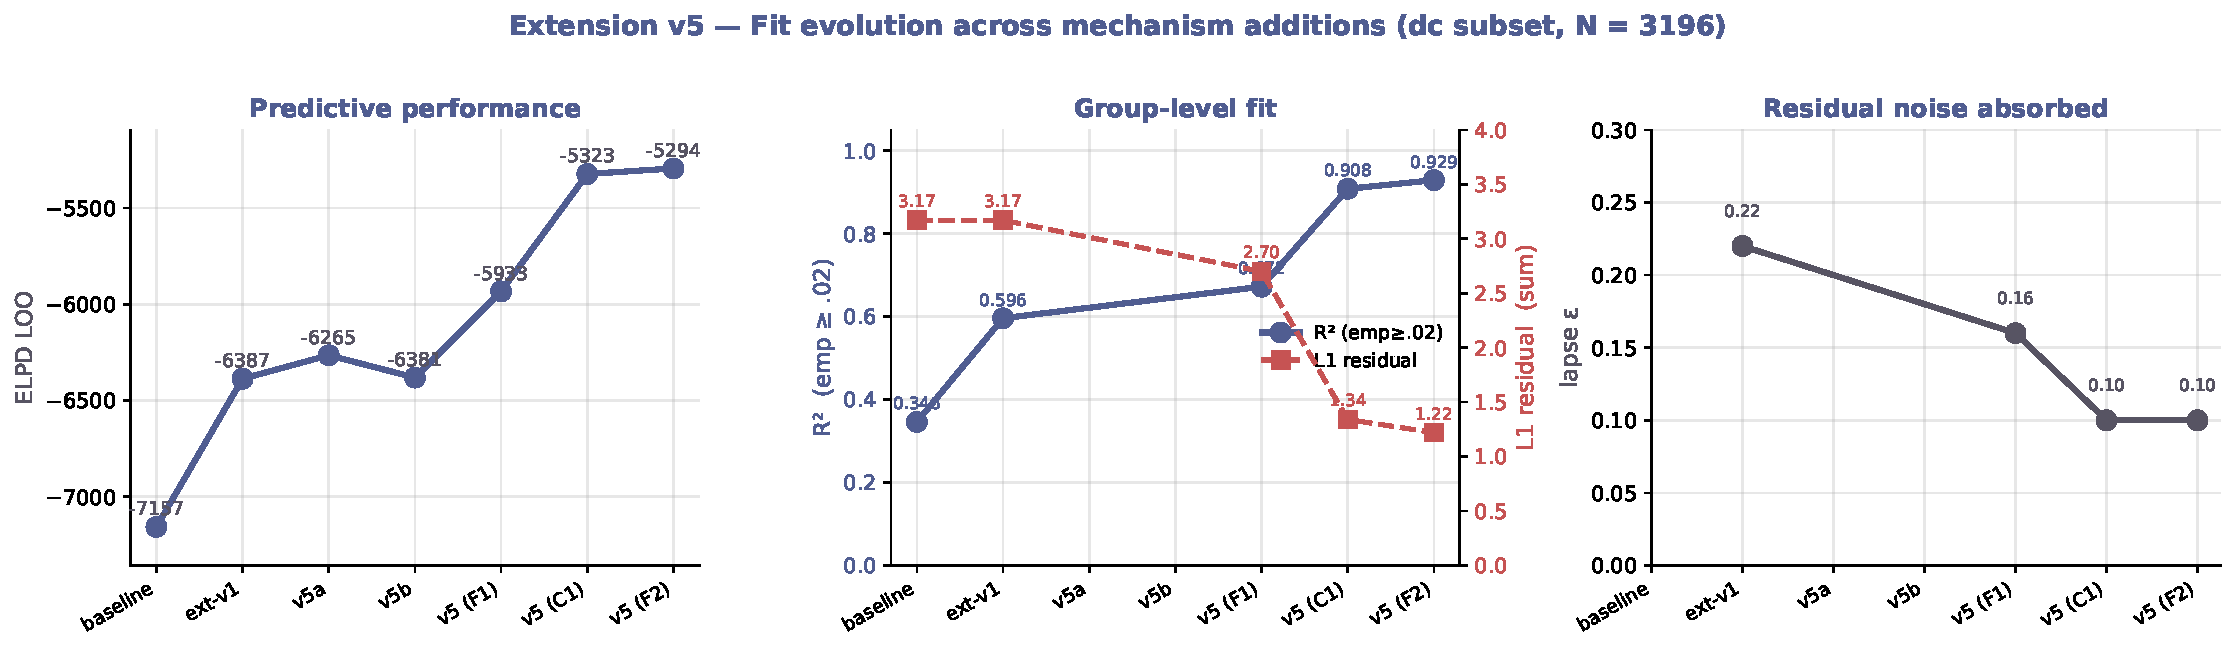
\includegraphics[width=0.97\linewidth]{v5_fit_evolution.pdf}
\end{center}
\vspace{-0.3em}
\footnotesize Each new mechanism shifts LOO and $R^2$ upward and $\varepsilon$ downward. v5b (sat $\gamma$ alone) flat vs ext-v1.
\end{frame}

% ====================================================================
\begin{frame}{Mechanism posteriors across stages}
\vspace{-0.3em}
\begin{center}
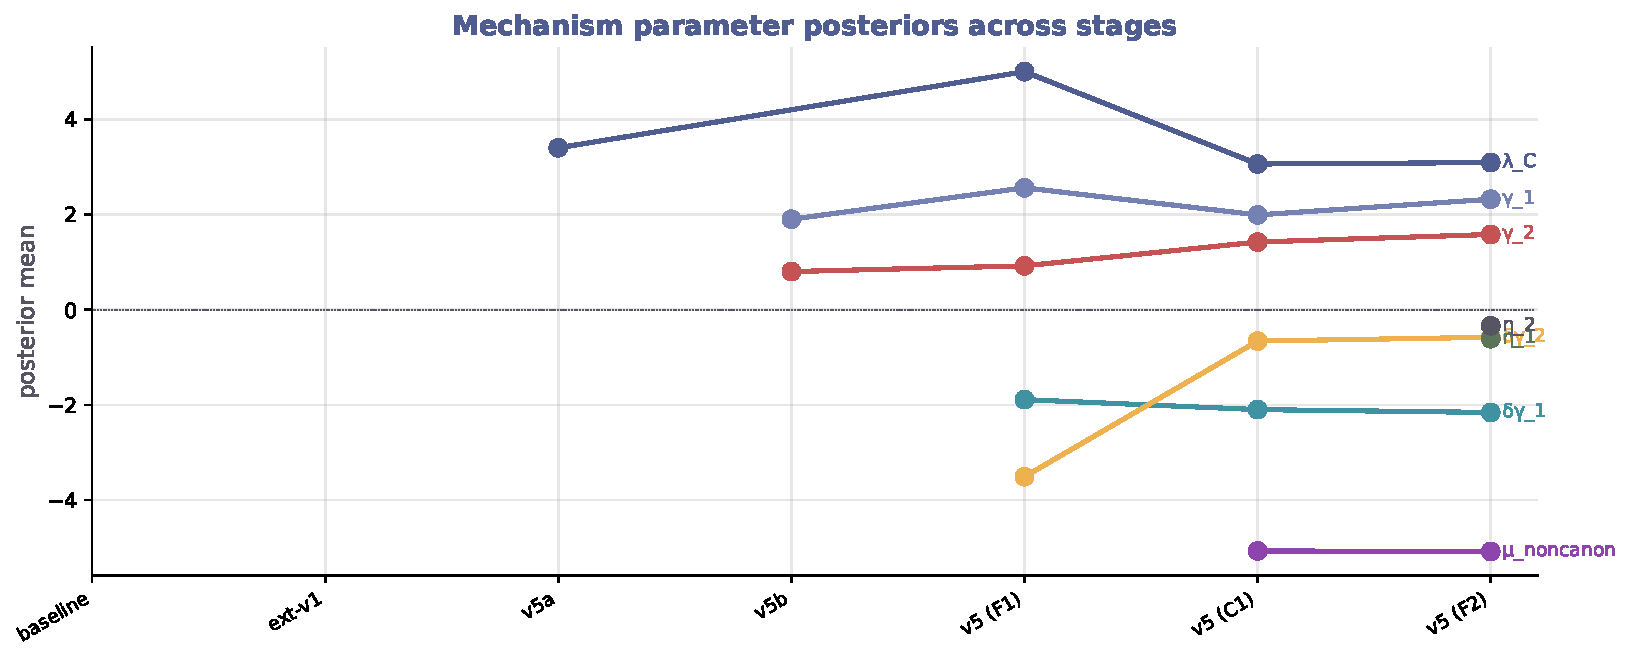
\includegraphics[width=0.97\linewidth]{v5_param_evolution.pdf}
\end{center}
\vspace{-0.3em}
\footnotesize Each parameter enters with a clear posterior sign and settles by F2. $\lambda_C$, $\mu_\mathrm{nc}$ strong; $\eta$ modest; $\delta\gamma_1$ strongly negative on csuff; $\delta\gamma_2$ shrinks once $\mu_\mathrm{nc}$ absorbs canonical-order variance.
\end{frame}

% ====================================================================
\begin{frame}{Full LOO \& fit record --- all stages}
\footnotesize
\begin{center}
\begin{tabular}{l rrrr rr}
\toprule
Stage & ELPD LOO & $\Delta$ vs baseline & $\Delta$ vs ext-v1 & $R^2$ & L1 & $\varepsilon$ \\
\midrule
baseline        & $-7157$ & $0$       & ---       & $.35$ & $3.17$ & ---   \\
ext-v1          & $-6387$ & $+770$    & $0$       & $.60$ & $3.17$ & $.23$  \\
\muted{v2 (first-word intercepts) --- rejected}  & $-6337$ & $+820$  & $+50$   & $.62$ & ---     & ---   \\
\muted{v3 (step-level $\mu$, per-dim $\alpha$) --- rejected} & \multicolumn{6}{l}{non-identifiable ($\hat R \leq 14.7$)} \\
\muted{v4 (step-level $\mu$, single $\alpha$) --- rejected} & $-6449$ & $+708$  & $-62$   & $.54$ & ---     & ---   \\
\acct{v5a ($\lambda_C$ only)}         & $-6265$ & $+892$  & $+122$   & ---   & ---     & ---   \\
\acct{v5b (sat.\ $\gamma$ only)}      & $-6381$ & $+776$  & $+6$     & ---   & ---     & ---   \\
\main{v5 (F1: $\lambda_C + \delta\gamma$)}   & $-5933$ & $+1224$ & $+454$   & $.67$ & $2.70$  & $.16$ \\
\main{v5 (C1: + $\mu_\mathrm{nc}$)}          & $-5323$ & $+1834$ & $+1063$  & $.91$ & $1.34$  & $.10$ \\
\emp{v5 (F2: + $\eta$)}                      & $-5294$ & $+1863$ & $+1093$  & $.94$ & $1.22$  & $.10$ \\
\muted{v5\_no\_lm (F3: F2 with $\beta=0$)}     & $-5314$ & $+1843$ & $+1073$  & $.92$ & $1.30$  & $.10$ \\
\bottomrule
\end{tabular}
\end{center}

\vspace{0.6em}
\begin{itemize}\itemsep0.15em
  \item LOO, $R^2$ (emp $\geq .02$), L1 (sum of $|\Delta|$ over 37 cells), $\varepsilon$ lapse posterior mean.
  \item \main{Baseline has no lapse and no length bias} --- $\gamma$ and $\varepsilon$ are \emph{hardcoded to $0$} in \texttt{likelihood\_function\_reported\_hier}, not sampled. All columns marked "---" are structurally absent, not just unreported.
  \item \emp{v2--v4}: rejected exploratory variants from memo \S4 --- see previous slide for reasons.
  \item v5a and v5b: isolated mechanism probes (no full R²/L1 reported in memo).
  \item Every add-on moves metrics monotonically in the right direction except v5b (sat $\gamma$ alone, null) and v4 (which made things worse than ext-v1).
  \item \main{F3 (LM prior removed)}: $-20$ ELPD vs F2 --- LM prior still contributes beyond $\mu_\mathrm{nc} + \gamma$. \emp{Keep it.}
\end{itemize}
\end{frame}

% ====================================================================
\begin{frame}{Ablation: is the LM prior still needed under F2?}
\small
\main{Test}: fit v5 (F2) with $\beta = 0$, effectively removing the LM prior. Every other mechanism identical.

\vspace{0.6em}
\begin{center}
\begin{tabular}{lrrrr}
\toprule
Model         & ELPD    & $\Delta$ vs F2 & $R^2$ & L1 \\
\midrule
\main{v5 (F2)}   & \main{$-5294$} & $0$     & \main{$.928$} & \main{$1.22$} \\
v5\_no\_lm (F3)  & $-5314$ & $-20.3$ & $.915$ & $1.30$ \\
\bottomrule
\end{tabular}
\end{center}

\vspace{0.6em}
\main{Posterior compensation when LM is removed:}
\begin{itemize}\itemsep0.15em
  \item $\lambda_C$: $3.09 \to 3.33$ (colour-boost works harder)
  \item $\gamma_2$: $1.58 \to 1.32$ (some 3-word preference re-absorbed)
  \item $\delta\gamma_1$: $-2.16 \to -2.39$ (more negative on csuff)
  \item $\mu_\mathrm{nc}, \gamma_1, \eta, \varepsilon$: essentially unchanged.
\end{itemize}

\vspace{0.6em}
\emp{Interpretation.} LM prior contributes $\sim\!20$ ELPD of residual signal the explicit mechanisms don't absorb. Likely encoding frequency structure beyond canonical ordering + length (e.g., relative frequency among same-shape canonical utterances). Getting a non-zero gap is actually reassuring --- it means $\mu_\mathrm{nc} + \gamma + \eta$ are capturing structure \emph{distinct} from the LM prior, not just refitting it.
\end{frame}

% ====================================================================
\begin{frame}{Full parameter record --- posterior means across stages}
\scriptsize
\begin{center}
\renewcommand{\arraystretch}{1.10}
\begin{tabular}{l cc cc ccccc}
\toprule
Parameter & baseline & ext-v1 & \muted{v2} & \muted{v4} & v5a & v5b & v5 (F1) & v5 (C1) & v5 (F2) \\
\midrule
$\alpha_D$           & single $\alpha$ & $6.92$ & $\sim 6.9$ & single $\alpha$ & $\sim 6.9$ & $\sim 6.9$ & hier. & hier. & hier. \\
$\alpha_C$           &                 & $1.85$ & $\sim 1.8$ &                 & $\sim 1.8$ & $\sim 1.9$ & hier. & hier. & hier. \\
$\alpha_F$           &                 & $1.89$ & $\sim 1.9$ &                 & $\sim 1.9$ & $\sim 1.9$ & hier. & hier. & hier. \\
\midrule
$\phi_C$ (first-word) & ---   & ---    & \emp{$-6.89$} & ---    & ---   & ---    & ---    & ---    & ---     \\
$\phi_F$ (first-word) & ---   & ---    & \emp{$-5.90$} & ---    & ---   & ---    & ---    & ---    & ---     \\
$\mu_C$ (step-level)  & ---   & ---    & ---    & fitted & ---   & ---    & ---    & ---    & ---     \\
$\mu_F$ (step-level)  & ---   & ---    & ---    & fitted & ---   & ---    & ---    & ---    & ---     \\
\midrule
$\lambda_C$           & ---   & ---    & ---    & ---    & \main{$+3.4$} & ---    & \main{$+5.0$} & \main{$+3.06$} & \main{$+3.09$} \\
$\gamma$ (linear)     & ---   & $2.31$ & $\sim 2$ & $\sim 2$ & ---   & ---    & ---    & ---    & ---    \\
$\gamma_1$            & ---   & ---    & ---    & ---    & ---   & $+1.9$ & $+2.56$ & $+1.99$ & $+2.32$ \\
$\gamma_2$            & ---   & ---    & ---    & ---    & ---   & $+0.8$ & $+0.92$ & $+1.42$ & $+1.58$ \\
$\delta\gamma_1$      & ---   & ---    & ---    & ---    & ---   & ---    & $-1.89$ & $-2.10$ & $-2.16$ \\
$\delta\gamma_2$      & ---   & ---    & ---    & ---    & ---   & ---    & $-3.51$ & $-0.66$ & $-0.58$ \\
$\eta_1$              & ---   & ---    & ---    & ---    & ---   & ---    & ---    & ---    & $-0.61$ \\
$\eta_2$              & ---   & ---    & ---    & ---    & ---   & ---    & ---    & ---    & $-0.34$ \\
$\mu_\mathrm{nc}$     & ---   & ---    & ---    & ---    & ---   & ---    & ---    & \emp{$-5.07$} & \emp{$-5.08$} \\
\midrule
$\log\beta$           & $\sim 2$ & $2.05$ & $\sim 2$ & $\sim 2$ & $\sim 2$ & $\sim 2$ & $2.05$ & $-0.18$ & $-0.17$ \\
$\varepsilon$         & ---   & $0.23$ & $\sim .2$ & $\sim .2$ & ---      & ---      & $0.16$ & $0.10$ & $0.10$ \\
$\tau$                & ---   & $0.92$ & ---    & ---    & ---   & ---    & $0.94$ & $0.60$ & $0.62$ \\
\bottomrule
\end{tabular}
\end{center}

{\scriptsize \muted{v3 omitted (non-identifiable). v2 / v4 columns show posterior means as reported in memo \S4.2 / \S4.4.}}


\vspace{0.6em}
\scriptsize
\begin{itemize}\itemsep0.1em
  \item \muted{"hier."} = $\alpha$ sampled hierarchically with per-participant $\delta_p$; population means close to ext-v1's values.
  \item Each new parameter enters with a clear, stable sign and keeps its sign across subsequent stages.
  \item $\log\beta$ drops sharply when $\mu_\mathrm{nc}$ is added --- canonical ordering absorbs what the LM prior was partially encoding.
  \item $\delta\gamma_2$ shrinks from $-3.51$ (F1) to $\sim\!-0.6$ (C1/F2) --- $\mu_\mathrm{nc}$ and $\eta$ absorb part of the 3-word-penalty work.
\end{itemize}
\end{frame}

% ====================================================================
\begin{frame}{Final v5 (F2) parameters --- full record}
\small
\begin{center}
\begin{tabular}{lllc}
\toprule
Parameter & Prior & Posterior mean (95\% CI) & $\hat R$\\
\midrule
$\alpha_D$           & HalfN(5)    & (hier.\ w/ $\delta_p$)  & $\leq 1.01$\\
$\alpha_C$           & HalfN(5)    & (hier.)                  & $\leq 1.01$\\
$\alpha_F$           & HalfN(5)    & (hier.)                  & $\leq 1.01$\\
\midrule
$\lambda_C$          & N(0,1)      & \main{$+3.09$} (2.67, 3.55) & 1.00\\
$\gamma_1$           & N(0,1)      & $+2.32$ (2.16, 2.49)     & 1.00\\
$\gamma_2$           & N(0,1)      & $+1.58$ (1.43, 1.74)     & 1.01\\
$\delta\gamma_1$     & N(0,1)      & $-2.16$ (-2.33, -1.97)   & 1.00\\
$\delta\gamma_2$     & N(0,1)      & $-0.58$ (-1.21, +0.04)   & 1.00\\
$\eta_1$             & N(0,1)      & $-0.61$ (-0.77, -0.43)   & 1.00\\
$\eta_2$             & N(0,1)      & $-0.34$ (-0.51, -0.15)   & 1.00\\
$\mu_\mathrm{nc}$    & N(0,1)      & \emp{$-5.08$} (-5.61, -4.56) & 1.01\\
\midrule
$\log\beta$          & N(0,0.5)    & $-0.17$                  & 1.00\\
$\varepsilon$        & Beta(1,50)  & \main{$0.10$} (0.09, 0.12) & 1.00\\
$\tau$               & HalfN(0.2)  & $0.62$ (0.51, 0.73)      & 1.00\\
\bottomrule
\end{tabular}
\end{center}
\end{frame}

% ====================================================================
\begin{frame}{PPC barplot --- baseline vs ext-v1 vs v5 (F2)}
\vspace{-0.5em}
\begin{center}
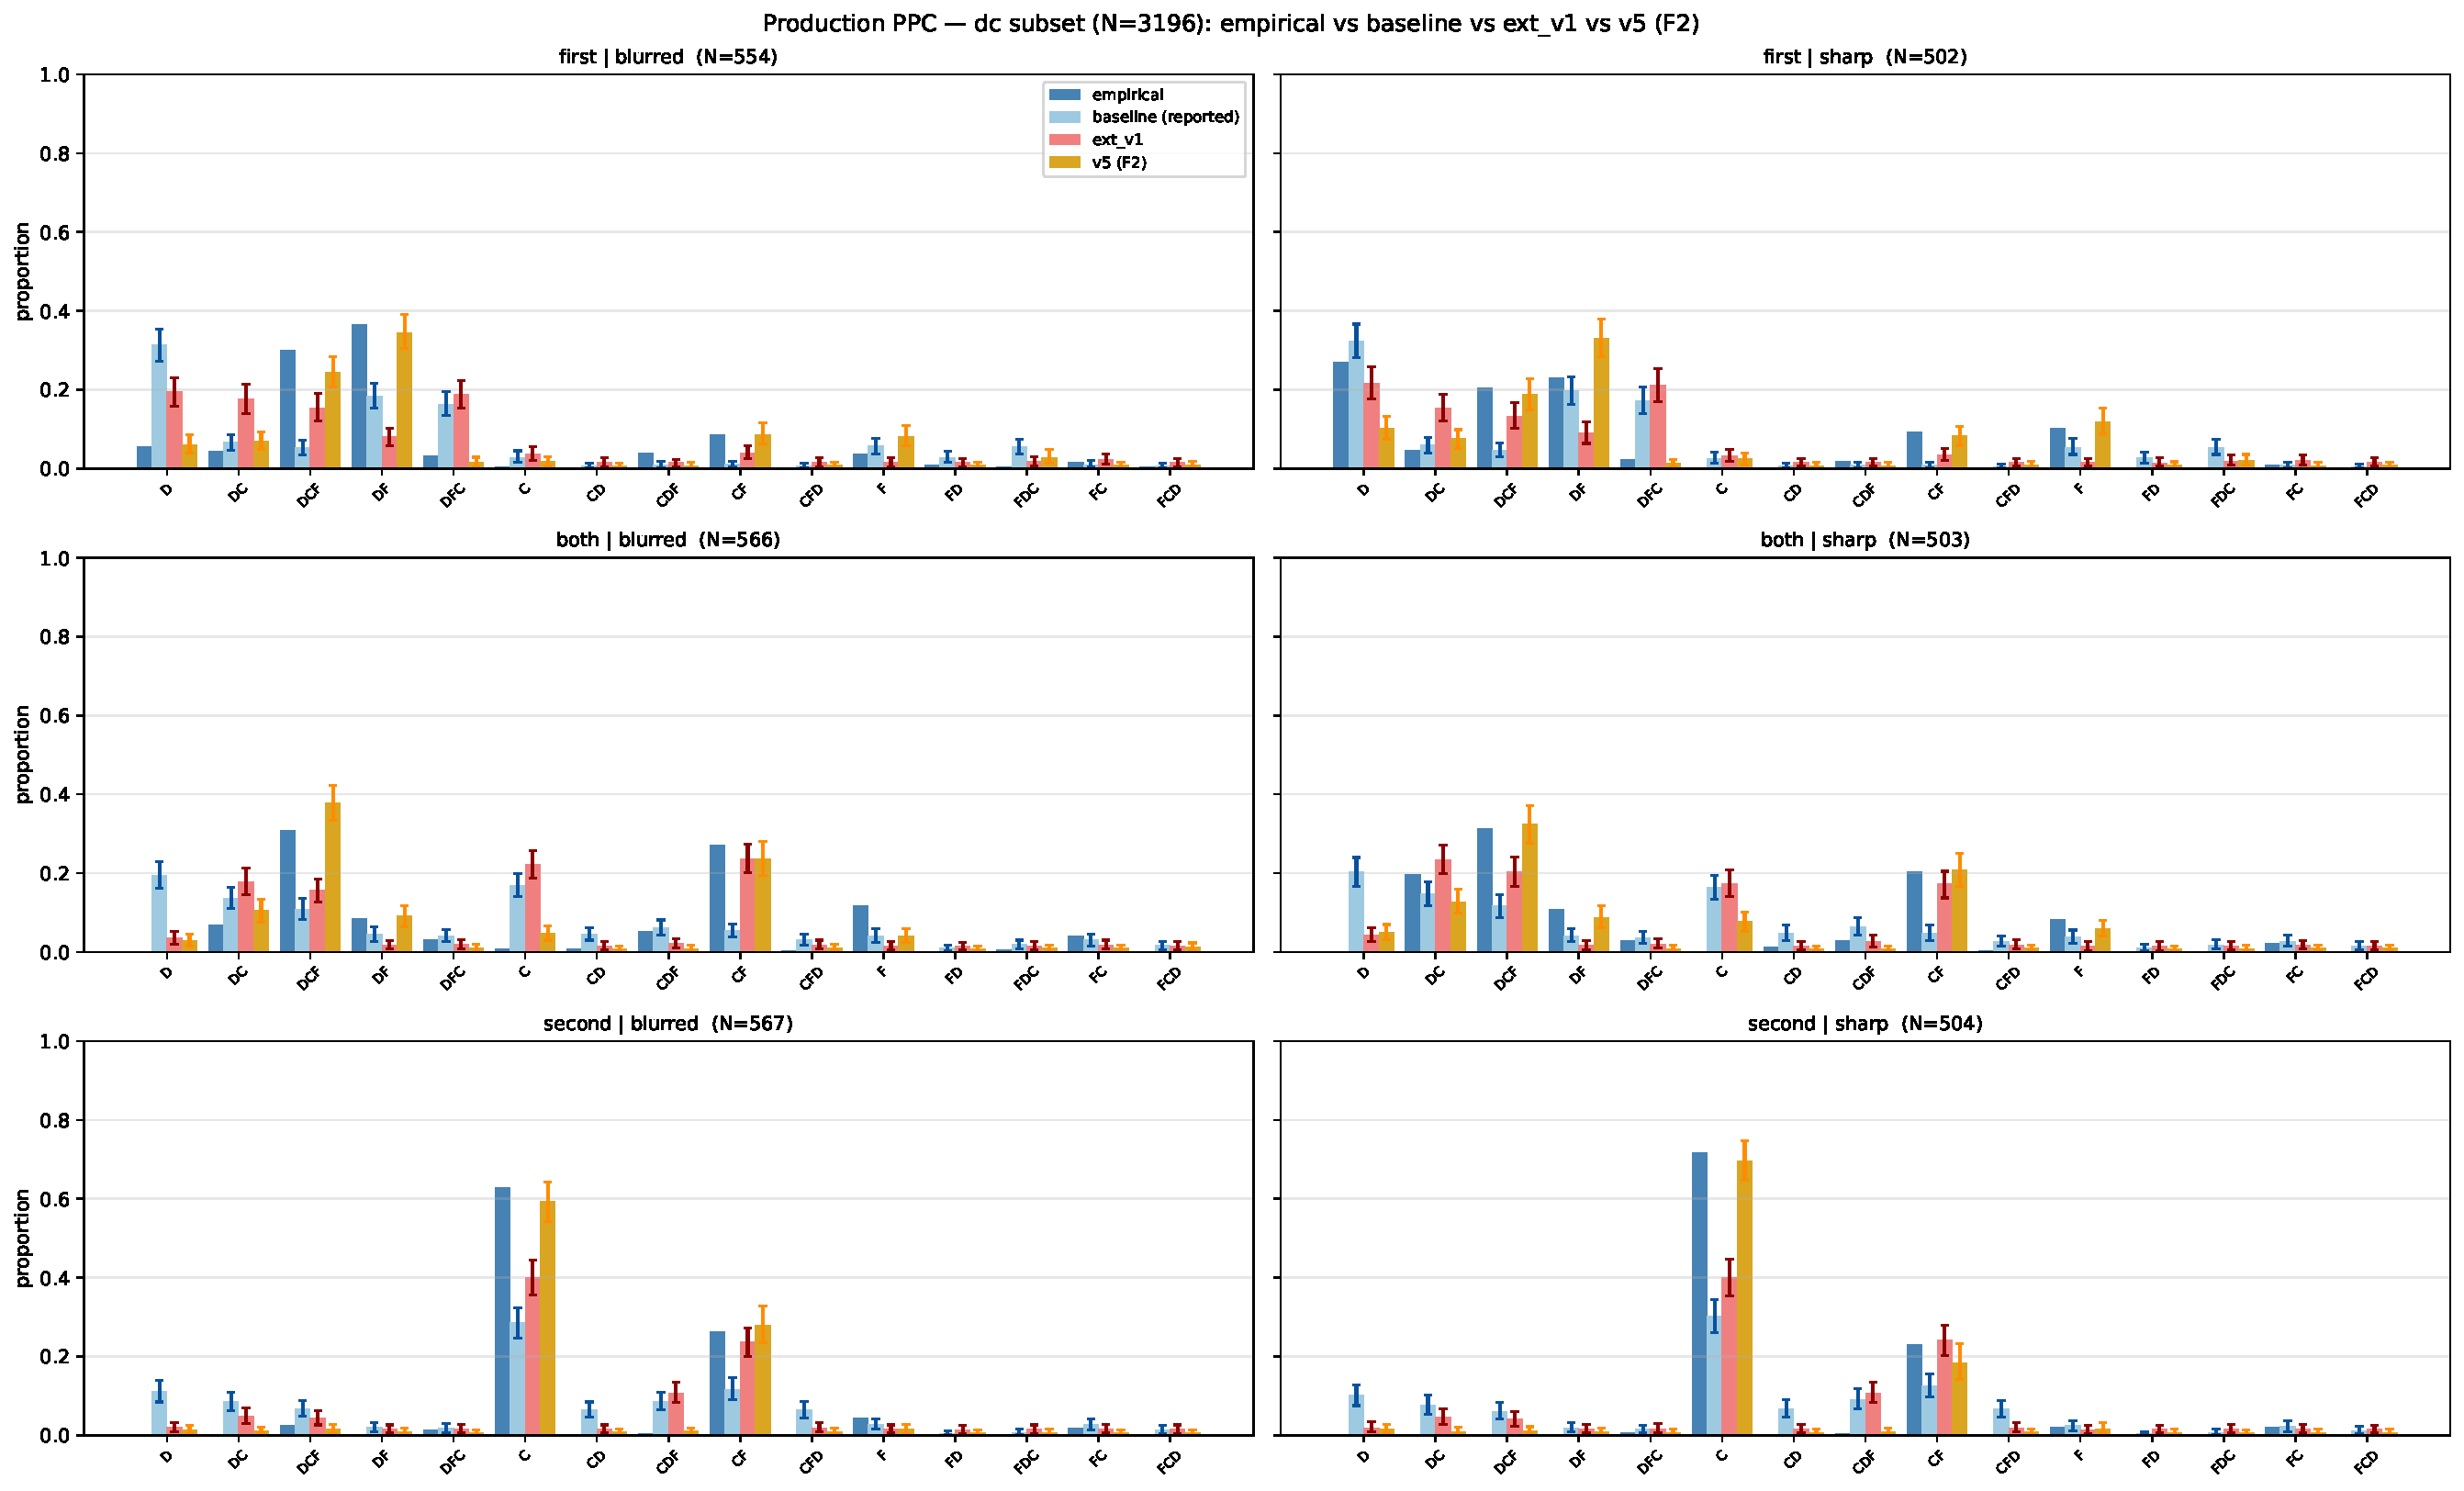
\includegraphics[width=0.98\linewidth]{production_ppc_barplot_v5_dc_F2.pdf}
\end{center}
\vspace{-0.3em}
\footnotesize Rows: \texttt{relevant\_property} (\acct{first} / \accg{both} / \accy{second}). Cols: sharpness.
\end{frame}

% ====================================================================
\begin{frame}{Predicted vs empirical ($n = 90$ cells)}
\vspace{-0.3em}
\begin{center}
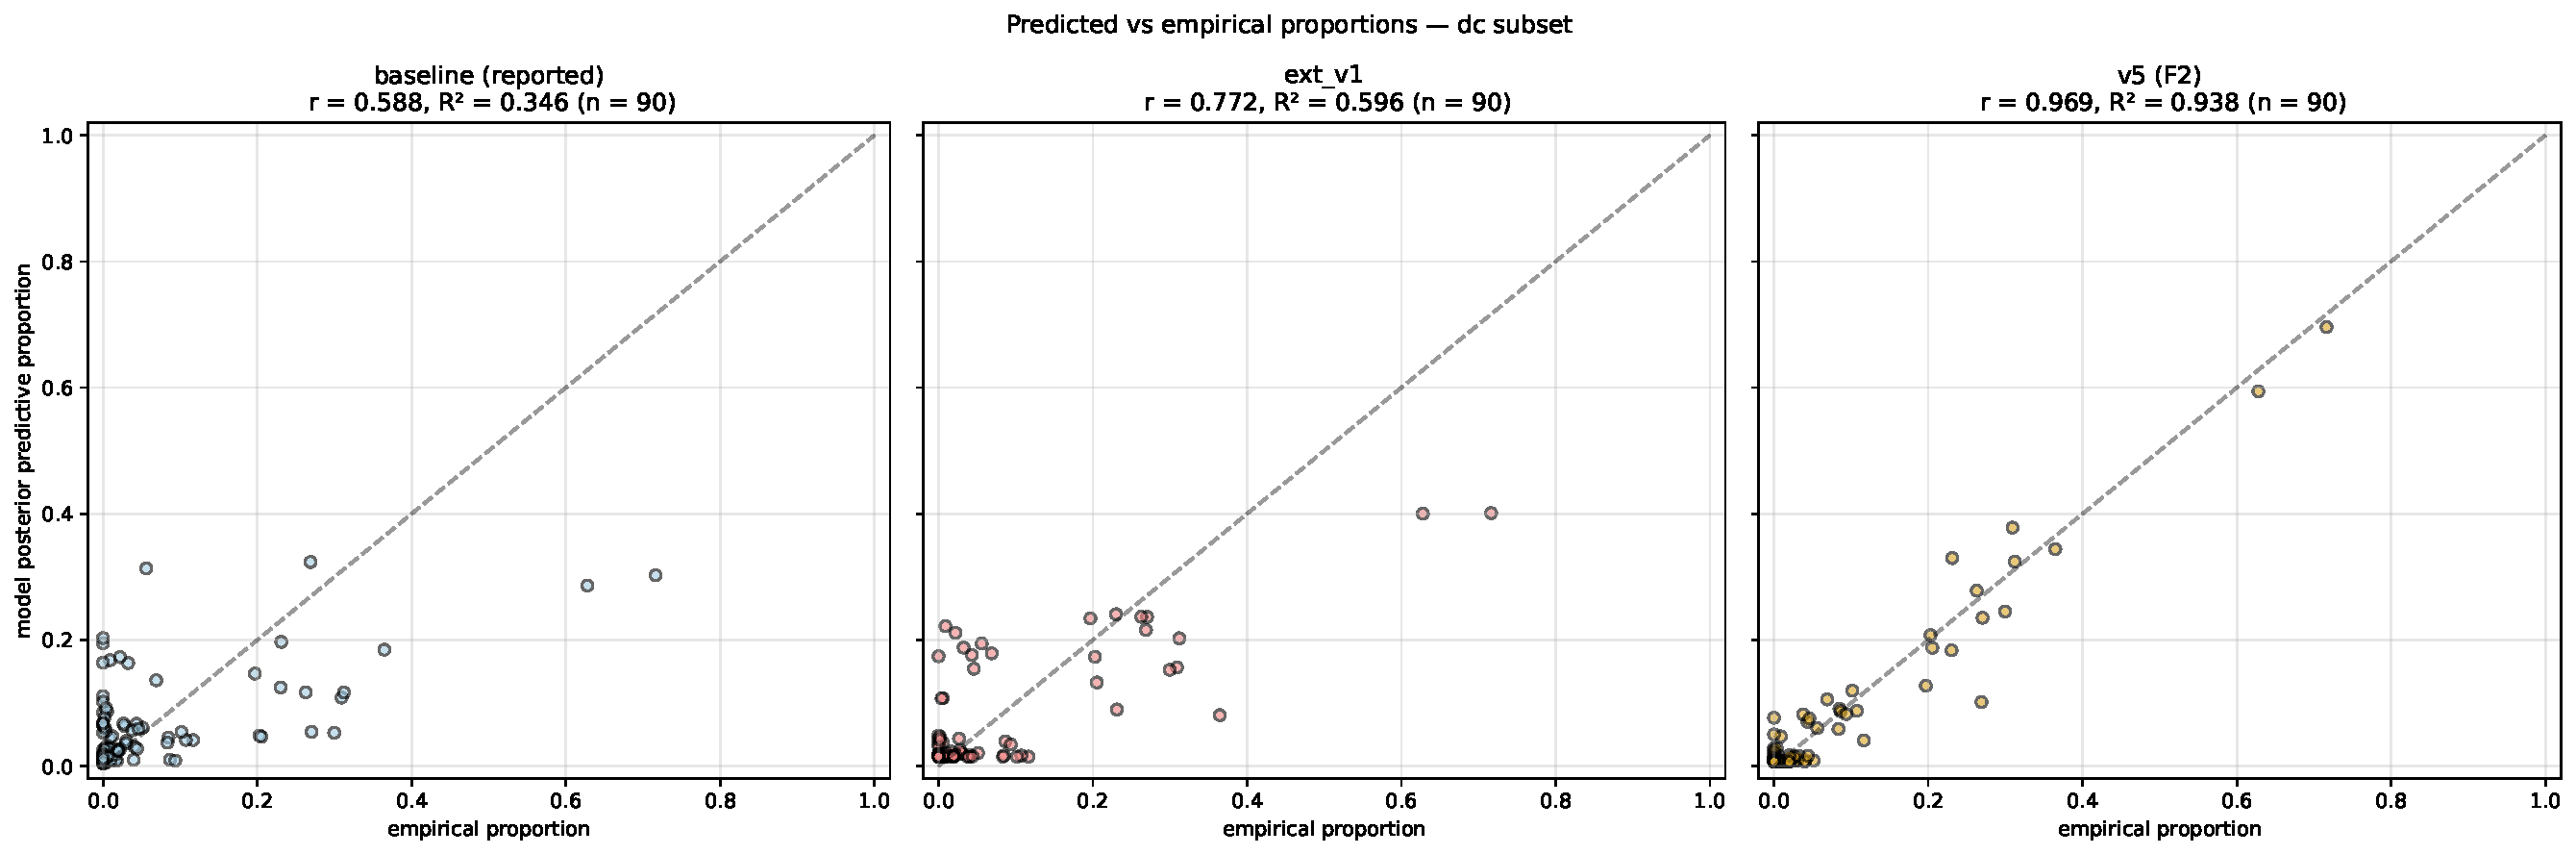
\includegraphics[width=0.98\linewidth]{production_correlation_v5_dc_F2.pdf}
\end{center}
\vspace{-0.3em}
\footnotesize $R^2$: baseline $.35 \to$ ext-v1 $.60 \to$ \main{v5 (F2) $.94$}.
\end{frame}

% ====================================================================
\begin{frame}{The $2\!\times\!2$ question: does the paper story survive?}
Under F2 mechanisms we re-ran the $2\!\times\!2$ (speaker architecture $\times$ semantics regime) on the dc subset.

\vspace{0.8em}
Three parameterisations to compare:
\begin{enumerate}\itemsep0.3em
  \item \main{Paper-reported (memo \S1)}: minimal, theory-driven.
  \item \main{F2-fixed globals}: global cells use $\gamma/\delta\gamma/\eta/\mu_\mathrm{nc}$ fixed at inc-recursive posterior means.
  \item \emp{F2-full globals}: every parameter sampled freely in every cell. Fairest comparison.
\end{enumerate}
\end{frame}

% ====================================================================
\begin{frame}{$2\!\times\!2$: paper-reported}
\begin{center}
\begin{tabular}{l|rr|r}
\toprule
             & recursive & static & $\Delta$(rec$-$sta) \\
\midrule
incremental  & $-7180$ & $-7199$ & \main{$+19$} ($\Delta/$dSE $= 10.28$) \\
global       & $-7628$ & $-7626$ & $-2$ (null) \\
\midrule
$\Delta$(inc$-$glb) & $+448$ & $+427$ & \\
$\Delta/$dSE        & $11.02$ & $11.08$ & \\
\bottomrule
\end{tabular}
\end{center}

\vspace{0.8em}
\main{Paper narrative}
\begin{itemize}\itemsep0.2em
  \item Architecture dominates: inc $\gg$ glb, $\Delta/$dSE $\approx 11$.
  \item Recursive helps incremental a lot, does not help global.
  \item Diff-in-diff $= +21$ (inc benefits more from rec).
\end{itemize}
\end{frame}

% ====================================================================
\begin{frame}{$2\!\times\!2$: F2 with globals' params \emph{fixed} at inc posterior means}
\begin{center}
\begin{tabular}{l|rr|r}
\toprule
              & recursive & static & $\Delta$(rec$-$sta) \\
\midrule
incremental   & $-5294$ & $-5297$ & $+2.80$ ($\Delta/$dSE $= 2.22$, marginal) \\
global (fixed)& $-5600$ & $-5619$ & \emp{$+19.15$} ($\Delta/$dSE $= 6.99$) \\
\midrule
$\Delta$(inc$-$glb) & $+306$ & $+323$ & \\
$\Delta/$dSE        & $10.51$ & $11.03$ & \\
\bottomrule
\end{tabular}
\end{center}

\vspace{0.8em}
\begin{itemize}\itemsep0.2em
  \item Architecture still dominant ($\Delta/$dSE $\approx 10.5$).
  \item \emp{Interaction has flipped}: rec now helps global, not incremental.
  \item But global's length/order parameters are \muted{fixed at inc values} --- unfair test.
\end{itemize}
\end{frame}

% ====================================================================
\begin{frame}{$2\!\times\!2$: F2 with globals \emph{fully sampled} --- the fair picture}
\begin{center}
\begin{tabular}{l|rr|r}
\toprule
             & recursive & static & $\Delta$(rec$-$sta) \\
\midrule
incremental  & $-5294$ & $-5297$ & $+2.80$ ($\Delta/$dSE $= 2.22$) \\
global (full)& $-5357$ & $-5365$ & $+8.25$ ($\Delta/$dSE $= 3.82$) \\
\midrule
$\Delta$(inc$-$glb) & $+63$ & $+69$ & \\
$\Delta/$dSE        & \emp{$3.18$} & \emp{$3.48$} & \\
\bottomrule
\end{tabular}
\end{center}

\vspace{0.8em}
\main{Key changes vs paper-reported}
\begin{itemize}\itemsep0.2em
  \item Architecture effect $\Delta/$dSE: $11 \to 3.2$ (\emp{$\sim\!1/3$ of paper's}).
  \item Regime-within-inc $\Delta/$dSE: $10.28 \to 2.22$ (\emp{$\sim\!1/5$ of paper's}).
  \item Regime-within-glb: $\approx 0 \to 3.82$ (\accg{appears, modestly}).
  \item Diff-in-diff: $+21 \to +5.45$ (same sign, small magnitude).
\end{itemize}
\end{frame}

% ====================================================================
\begin{frame}{Full record --- side-by-side}
\small
\begin{center}
\begin{tabular}{lccc}
\toprule
                             & Paper        & F2-fixed & \main{F2-full} \\
\midrule
$R^2$ (all cells)            & $.35$      & $.94$ & $.94$ \\
L1 residual                  & $3.17$    & $1.22$   & $1.22$ \\
Lapse $\varepsilon$          & $0.22$      & $0.10$ & $0.10$ \\
\midrule
Arch effect $\Delta/$dSE     & $\pm 11$    & $\pm 10.5$ & $\pm 3.2$ \\
Regime $|$inc $\Delta/$dSE   & $10.28$     & $2.22$ & $2.22$ \\
Regime $|$glb $\Delta/$dSE   & $\approx 0$ & $6.99$ & $3.82$ \\
Interaction (diff-in-diff)   & $+21$       & $-16$ & $+5.45$ \\
\midrule
Rec helps\ldots              & incremental & global (artefact) & slightly global \\
\bottomrule
\end{tabular}
\end{center}
\end{frame}

% ====================================================================
\begin{frame}{The tradeoff}
\begin{columns}[t]
\begin{column}{0.48\textwidth}
\main{Theory track (paper)}
\begin{itemize}\itemsep0.2em
  \item Minimal, motivated mechanisms
  \item Clear $2\!\times\!2$ interaction
  \item \emp{Poor group-level fit ($R^2 = .35$)}
  \item \emp{Seven large misfits in \S5.3}
  \item Lapse absorbs unexplained structure
\end{itemize}
\end{column}

\begin{column}{0.48\textwidth}
\accy{Mechanism track (F2)}
\begin{itemize}\itemsep0.2em
  \item Rich; each term literature-grounded
  \item Excellent fit ($R^2 = .94$)
  \item All seven misfits resolved
  \item Lapse halved ($0.22 \to 0.10$)
  \item \emp{Architecture signal shrinks to $\Delta/$dSE $= 3$}
  \item \emp{Regime-within-inc weakens to marginal}
\end{itemize}
\end{column}
\end{columns}

\vspace{1em}
\main{Core tension.} Mechanisms designed to reduce residuals explain variance that the paper's minimal parameterisation attributed to \emp{architecture $\times$ regime}. The interaction survives in reduced form.
\end{frame}

% ====================================================================
\begin{frame}{Two readings}
\small
\main{Reading I: mechanisms as rivals}

The paper's interaction was partly \emph{architectural sparsity fitting error structure}. Once error is absorbed by explicit mechanisms (colour salience, canonical ordering, context-dep.\ length), the residual architectural signal is modest. The main claim must weaken.

\vspace{1em}
\accy{Reading II: mechanisms as scaffolding}

$\lambda_C$, $\mu_\mathrm{nc}$, $\delta\gamma$, $\eta$ are \emph{implementations} of what context-updating $\times$ incremental architecture is \emph{supposed} to do. Of course adding them absorbs architectural signal --- they are the phenomena the architecture was indirectly capturing.

\vspace{1em}
\emp{Both are defensible. The choice shapes the paper's framing.}
\end{frame}

% ====================================================================
\begin{frame}{Four concrete decisions}
\begin{enumerate}\itemsep0.4em
  \item \main{Report v5 (F2) or keep the paper-reported model?}\\
  \small A middle path: main-text keeps the reported model; supplementary section shows F2 as mechanism-level refinement.

  \item \main{If we adopt F2, how do we frame the interaction?}\\
  \small Reading I softens; Reading II preserves. A referee will ask.

  \item \main{Adopt the corrected \texttt{COLOUR\_SUFFICIENT} flag $(ercf, zrdc)$?}\\
  \small Independent of the F2 decision. Probably yes --- the definition is simply more accurate.

  \item \main{Generalise beyond the dc subset?}\\
  \small Parallel runs on df (size+form) and cf (colour+form) would test whether F2 mechanisms are symmetric or colour-specific.
\end{enumerate}
\end{frame}

% ====================================================================
\begin{frame}{Open questions}
\small
\begin{itemize}\itemsep0.4em
  \item \main{Strategy heterogeneity.} $\varepsilon = 0.10$ is smaller than ext-v1's $0.22$ but non-zero. The \texttt{first/sharp} bare-\texttt{D} vs \texttt{DF} split looks like two participant sub-populations.
  \item \main{Full-data ($N = 9586$) run.} Our early full-data run used the incorrect flag. A clean full-data F2 run would take $\sim\!15$ min on GPU.
  \item \main{df and cf subsets.} Do the mechanisms generalise? If a ``form-sufficient'' flag is needed, symmetric structure; if not, colour-specificity.
  \item \main{LOO warnings.} \texttt{az.compare} flagged Pareto $k > 0.7$ in some cells. Differences reliable in direction, noisier in magnitude.
\end{itemize}
\end{frame}

% ====================================================================
\begin{frame}{Summary}
\small
\begin{itemize}\itemsep0.3em
  \item Paper-reported model: theory-driven, interpretable $2\!\times\!2$, but $R^2 = .35$.
  \item Residuals trace to three independent phenomena: \main{colour salience}, \main{canonical ordering}, \main{condition-dependent length bias}.
  \item Adding all three (v5 F2) lifts fit to $R^2 = .94$ and lapse to $.10$, with every new parameter informative, 0 divergences.
  \item Re-running the $2\!\times\!2$ under F2 with \emp{freely sampled} globals: architecture effect shrinks $\sim\!3\times$; regime effect shrinks and partially flips direction.
  \item Two readings of the tradeoff; both defensible.
  \item Decision the paper needs: \emp{report F2, report paper-reported, or both?}
\end{itemize}

\vspace{1em}
\muted{Artefacts: branch \texttt{feat/extension-v5},
spec at \texttt{docs/superpowers/specs/...},
synthesis at \texttt{10-writing/extension\_v5\_synthesis.md}.}
\end{frame}

% ====================================================================
\begin{frame}{Thanks}
\centering
\vspace{2em}
\Large Questions and discussion.

\vspace{2em}
\normalsize
\begin{tabular}{ll}
\texttt{feat/extension-v5} & 16 commits \\
\texttt{10-writing/extension\_v5\_synthesis.md} & detailed write-up \\
\texttt{10-writing/extension\_v5\_slides\_csp.tex} & this deck \\
\texttt{05-modelling-production-data/figures/v5/} & figures used above \\
\texttt{05-modelling-production-data/results/} & LOO + residual CSVs \\
\end{tabular}
\end{frame}

\end{document}
